


\chapter{Measurement of \texorpdfstring{$tq\gamma$}{tqGamma}}
\label{chap:measurement}

\section{The ATLAS Experiment}
\label{sec:atlas}
\begin{figure}
    \centering
    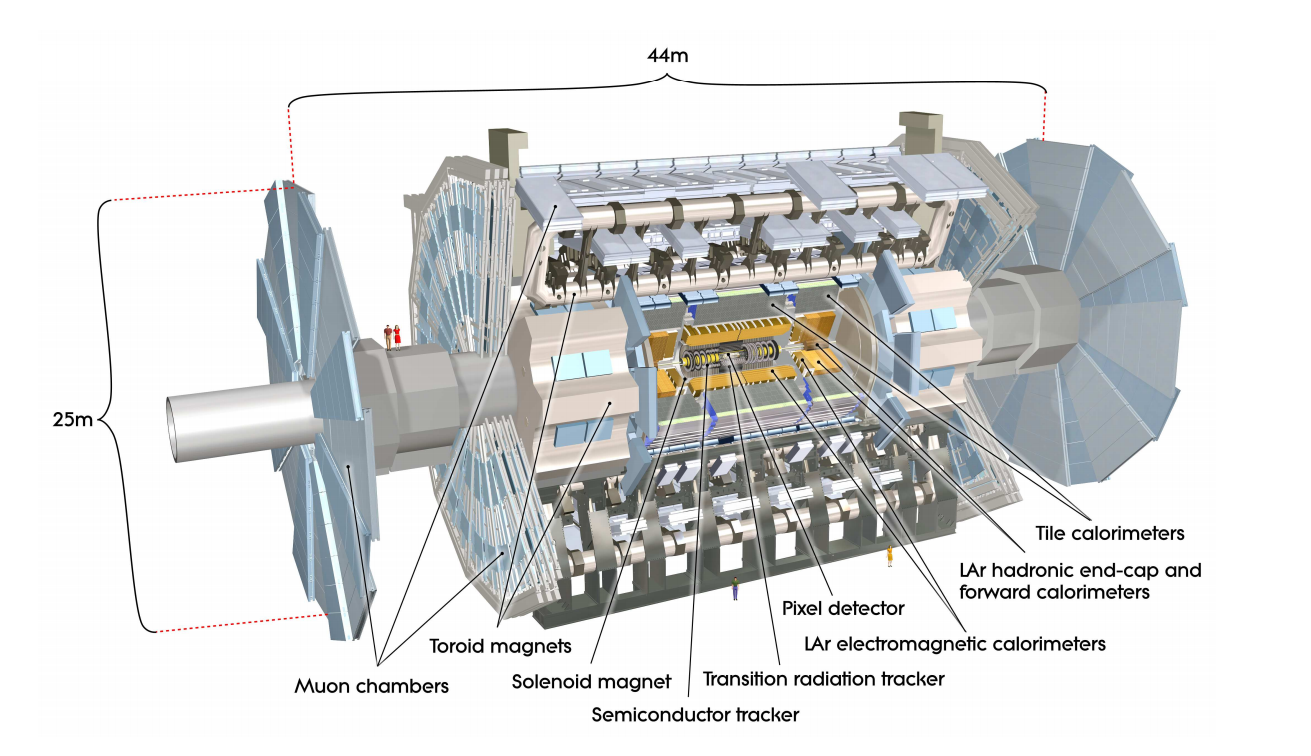
\includegraphics[width=0.9\textwidth]{Plots/atlasSCHEMA.PNG}
    \label{fig:atlasschema}
    \caption{Schematic visualisation of the ATLAS Detector \cite{Collaboration_2008}.}
\end{figure}

The European Organization for Nuclear Research, known as CERN, located in Geneva, has various experiments studying elementary particles through the collision of mainly heavy ions and protons. 
The Large Hadron Collider (LHC), the largest particle accelerator of CERN \cite{LHC}, has a circumference of $27 \,\si{\kilo\metre}$ and can collide particles with a center of mass energy of up to $\sqrt{s} = 13 \,\si{\tera\electronvolt}$. 


The LHC consists of four main experiments: the ALICE, the LHCb, the CMS and the ATLAS experiments \cite{Collaboration_2008}. The research in this thesis is done with the help of the largest of these experiments, the ATLAS experiment. Figure 1 visualizes the structure of the ATLAS detector. 
A coordinate system needs to be defined in order to discuss the construction of the experiment and positions of objects. Three different coordinates are used to describe positions inside the detector: First, the azimuthal angle $\phi$, which ranges from $0$ to $2\pi$. 
Next, the pseudorapidity $\eta$, which is defined to be $\eta = -\ln(\tan \theta)$, where $\theta$ is the angle to the beam axis. The smaller $\theta$ is, the higher the pseudorapidity. And lastly, a distance $\Delta R$, which can be defined in the $\phi$-$\theta$-plane as $\Delta R = \sqrt{(\Delta \phi)^2 +(\Delta \eta)}$.

The ATLAS detector is built symmetrically around the particle beam and can be divided into three subdetectors:

The inner detector \cite{innerdetector} tracks charged particles just after the collision. 
It consists of three different systems of sensors in a magnetic field parallel to the beam. 
These sensors are the pixel detector, the semiconductor tracker and a transition radiation tracker to track particles with gas-filled tubes. 

In the EM calorimeter, metal layers (tungsten, copper or lead) absorb incoming particles and convert them into lower-energy particles called a shower \cite{EMCal}. The calorimeters detect showers produced by electrons (and positrons), photons and hadrons. The barrel part of this calorimeter covers the pseudorapidity range $|\eta| < = 1.475$ and the end-cap components cover $1.375 <|\eta|< 3.2$.
Hadrons do not deposit all of their energy into the EM calorimeter; their showers get absorbed by steel layers in the hadronic calorimeter \cite{HADCal} behind the EM calorimeter. 
Here, plastic scintillating tiles produce photons that get converted into an electric current. The scintillating tiles cover the region $|\eta| < 1.7$. The region $1.5 < |\eta| < 4.9$ is then used by the cooper + liquid argon and tungsten + liquid argon calorimeter.

The muon spectrometer measures trajectories of muons with the help of a magnetic field. Muons are the only detectable particles that pass through all inner detector elements without losing a lot of energy. The spectrometer detects muons in the range of $\bigl|\eta\bigr| < 2.7$. 
Monitored drift tubes measure pseudorapidities up to $|\eta| = 2.0$ and cathode strip chambers cover higher pseudorapidities.  



\section{Object Reconstruction at the ATLAS experiment}
\label{sec:reconstruction}
\subsection{Reconstruction of photons}
\label{sec:reconphoton}

Photons mostly do not leave tracks inside the inner detector. They are reconstructed from clusters in the electromagnetic calorimeter \cite{EMCal}. Photon candidates need to pass the $Tight$ identification \cite{TightLH} criteria with the transverse momentum being $p_T >20\,\si{\giga\electronvolt}$ and $|\eta| < 2.3$. 
Photon candidtaes in the calorimeter transition region $1.37 < |\eta| < 1.52$ are exclused. 

\subsection{Reconstruction of electrons and muons}
\label{sec:reconlepton}

Leptons like an electron also produce clusters inside the electromagnetic calorimeter and leave charged particle tracks in the inner detector. All leptons in the calorimeter region $1.37 < |\eta| < 1.52$ are excluded. Electron candidates have to pass the tight likelihood identification (TightLH \cite{TightLH}) conditions of $p_T > 27 \,\si{\giga\electronvolt}$ and $|\eta| < 2.47$. 
To reconstruct muons, charged particle tracks in the inner detector are matched with muon spectrometer tracks. Muon candidates are required to pass the Medium identification \cite{Medium} with $p_T > 27 \,\si{\giga\electronvolt}$ and $|\eta| < 2.5$.

\subsection{Jets}
\label{sec:jets}
Jets are showers of mostly mesons and fewer baryons in the hadronic calorimeter that result from the production of high energy quarks (colour confinement). They deposit some of their energy in calorimeter cells which then are combined into clusters by the anti-$k_t$ algorithm \cite{anti_k_t} with a radius parameter of $R = 0.4$. 
It is then required that the cluster has a transverse momentum of $p_T > 25 \,\si{\giga\electronvolt}$ and $\bigl|\eta\bigr| < 4.5$. If these conditions are met, the cluster is identified to be a jet.

Detector noise can lead to the misidentification of a jet. The nature of these misidentified jets has been studied thoroughly and a so-called "jet cleaning procedure" is used to tag them. 
Any event containing at least one "bad" jet is removed by the algorithm \cite{jetclean}. 
\subsection{b-tagging}
\label{sec:btagging}

For the measurement of $tq\gamma$, the identification of jets produced by bottom quarks ($b$-taggigng) must be made with high accuracy to distinguish $bottom$ jets from $charm$ jets. Here, the $DL1r$ algorithm is implemented for $b$-tagging. 
Only jets passing $70\%$ working point and $p_T >20 \,\si{\giga\electronvolt}$ are viewed as $b$-jets in this analysis. 
Detailed information on the $DL1r$-algorithm can be found in the references \cite{btag1} and \cite{btag2}.

\subsection{Missing transverse momentum \texorpdfstring{$E_T^{\text{miss}}$}{}}

If all particles originating from the hard-scattering process are measured, there should be no magnitude for the sum of the transverse momentum $p_T$ of all particles. 
Any measured magnitude is therefore attributed to an unmeasured particle. The missing transverse energy $E_T^{\text{miss}}$ is consequently defined as the negative of this sum and assinged to a neutrino, as neutrinos pass through detectors without losing practically any energy and therefore are undetectable in this experiment.

\subsection{Short note on the reconstruction of the top quark}

The missing transverse momentum $E_T^{\text{miss}}$ is used to reconstruct the neutrino in the $tq\gamma$ process. Here, the $z$ component of the neutrino's momentum is derived by requiring the invariant mass of the neutrino and the leading lepton to be equal to the $W$ boson mass.
The top quark is then reconstructed by combining the resulting four-momentum of the neutrino and the four-momenta of the lepton candidate and the $b$-jet \cite{toprecon}.  
\section{Background contributions from similar processes}



Various processes besides $tq\gamma$ are also accepted by the criteria for event selection \ref{sec:eventselect}. Contributions from these processes are considered background. 
Some background processes consist of "real" photons while a photon in other background processes are misreconstructed. 
The process $t\bar{t}\gamma$, the pair production of the top quark with a photon, holds the most similar final state. This process does have an additional $b$-jet because of the second top quark, but it may not get $b$-tagged correctly. If the decay of the other top quark also does not get correctly reconstructed, then the $t\bar{t}\gamma$ process virtually looks identical to $tq\gamma$. 
Next highest background contributions come from the production of a $W$-boson with a photon and jets, a $Z$-boson with a photon jets and $t\bar{t}$, which has a "faked" photon.

Table \ref{tab:background} lists these and more of these processes contributing to the background.
\begin{table}
    \centering
    \begin{tabular}{c c c}
        \toprule
        {} & Process & Explanation\\
        \midrule
        1 & $tq\gamma$&         Single top+photon production\\[.1cm]
        2 & $t\bar{t}\gamma$&   Top pair production with photon\\[.1cm]
        3 & $W\gamma + jets$&   Production of W boson with a photon and jets\\[.1cm]
        4 & $Z\gamma + jets$&   Production of W boson with a photon and jets\\[.1cm]
        5 & $t\bar{t}$&         Top pair production\\[.1cm]
        6 & $s\text{-}chan$&    $s$-channel single top production (see Section \ref{sec:tqgammainsm})\\[.1cm]
        7 & $t W$&              $tW$-channel single top production (see Section \ref{sec:tqgammainsm})\\[.1cm]
        8 & $t\text{-}chan$&    $t$-channel single top production (see Section \ref{sec:tqgammainsm})\\[.1cm]
        9 & $VV$&               Diboson production\\[.1cm]
        10& $W+jets$&           Production of W boson alongside jets\\[.1cm]
        11& $Z+jets$&           Production of Z boson alongside jets\\[.1cm]
        \bottomrule
    \end{tabular}
    \caption{List of SM processes that contribute to background in the measurement of $tq\gamma$.}
    \label{tab:background}
\end{table}





